\section{Auswertung}
\label{sec:Auswertung}

\subsection{Magnetfeldkalibrierung}

Wie schon in der Durchführung erklärt, wird im ersten Versuchsteil das Magnetfeld
mittels Hallsonde in Abhängigkeit vom Betriebsstrom des Elektromagneten gemessen.
Die Messwerte dazu sind in Tabelle \ref{tab:kalib} aufgezählt.
Aufgrund von Messungenauigkeiten durch manuelles Messen mit der Hallsonde wird ein Fehler von $\SI{50}{\milli\tesla}$
bei den Magnetfeldwerten angenommen. Außerdem wird ein Ablesefehler von $\SI{0.5}{\ampere}$ für
die Stromstärke berücksichtigt. Die Messwerte mit den entsprechenden Fehlern sind in
Abbildung \ref{fig:kalib} graphisch aufgetragen. Es wird ein linearer Fit zur Funktion
\begin{align}
  B(I) = m \cdot I + b
\end{align}
durchgeführt, bei welchem sich die Parameter
\begin{align}
  m &= \SI{5.39(16)e01}{\milli\tesla\per\ampere} \\
  b &= \SI{42(19)}{\milli\tesla}
  \label{eqn:kalibparams}
\end{align}
ergeben. Mit diesen Parametern kann in den Folgeschritten das Magnetfeld an der Cd-Lampe aus der
eingestellten Stromstärke ermittelt werden.

\begin{figure}[H]
  \centering
  \includegraphics{build/kalibrierung_b.pdf}
  \caption{Magnetfeldmesswerte $B$ in Abhängigkeit von der Stromstärke $I$ und linearer Fit der Messwerte.}
  \label{fig:kalib}
\end{figure}

\subsection{Ausmessung der roten Spektrallinien}
\label{sec:rotspektr}

Im nächsten Schritt wird nach erfolgreicher Justage ein Kamerabild der roten Spektrallinie
bei ausgeschaltetem Magnetfeld aufgenommen. Mit Hilfe des Zeichenprogramms \textit{inkscape} wird dieses Bild
bearbeitet um die Abstände zwischen den Linien verschiedener Ordnung zu ermitteln. Das bearbeitete Bild
kann in Abbildung \ref{fig:redB0} eingesehen werden.

\begin{figure}[H]
  \centering
  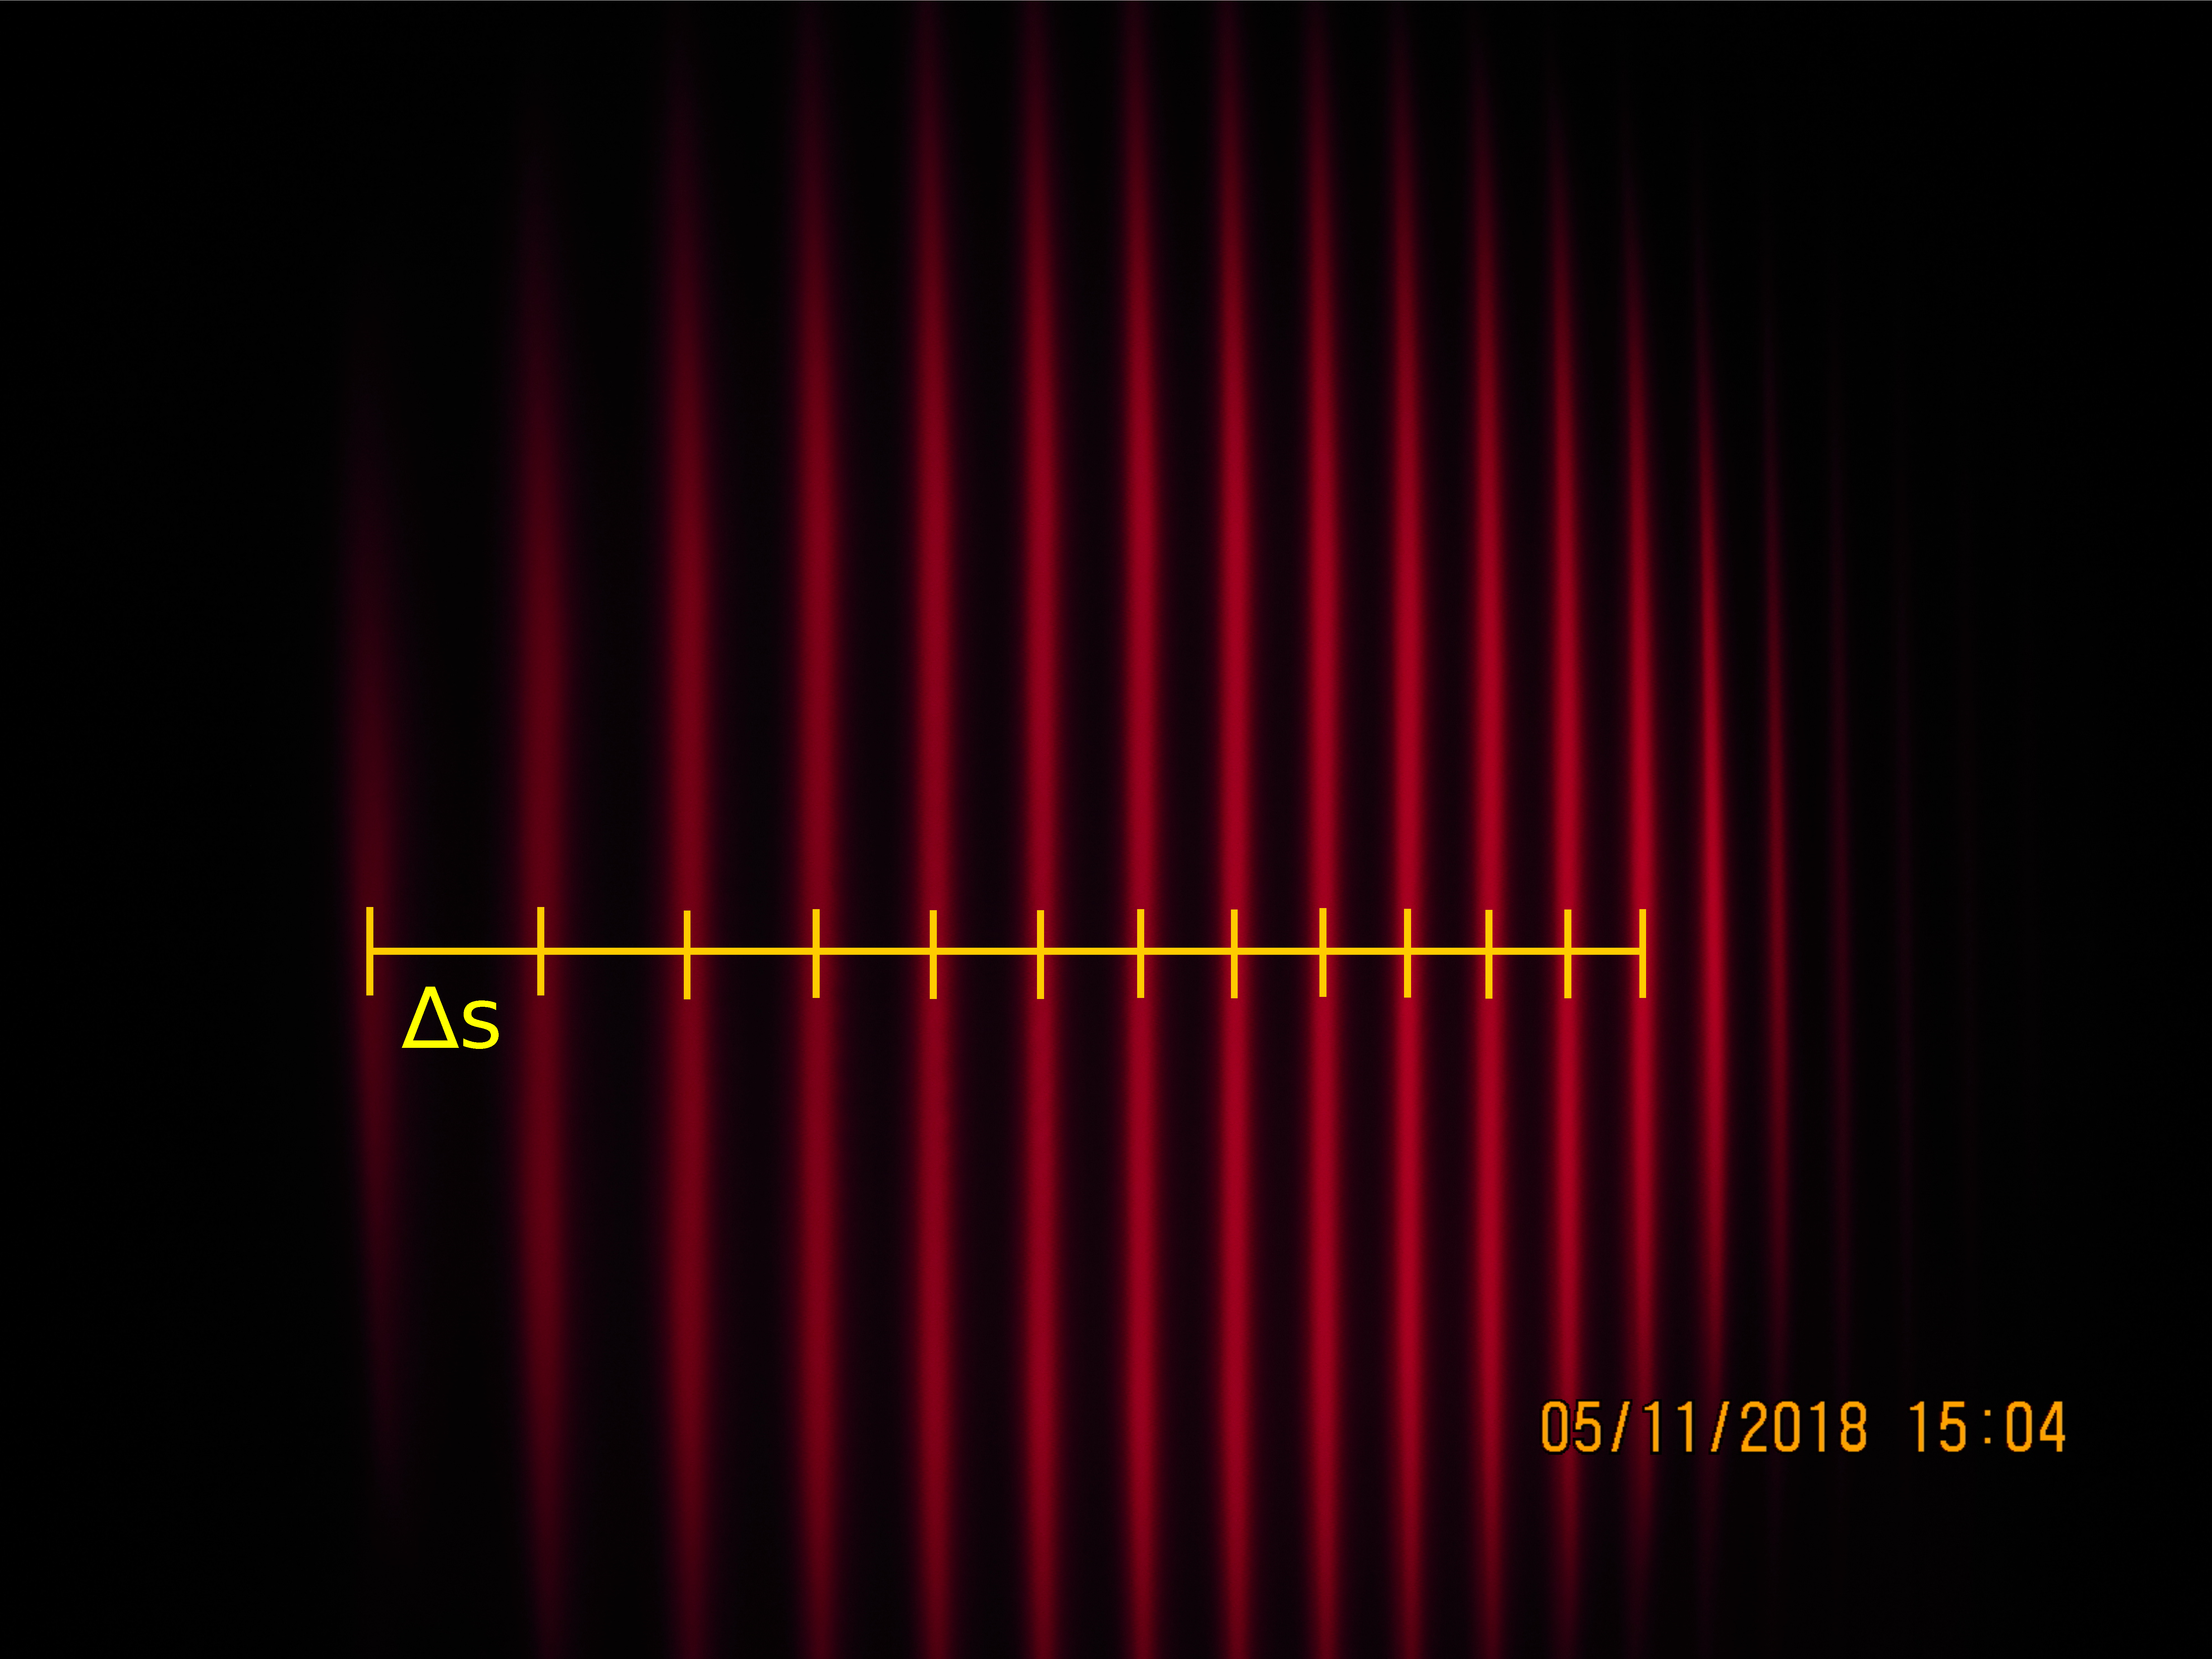
\includegraphics[height=8cm]{Experimental Pictures/red_norm.pdf}
  \caption{Kamerabild der roten Spektrallinie bei ausgeschaltetem Magnetfeld. \textit{bearbeitet}}
  \label{fig:redB0}
\end{figure}

Die gemessenen Abstände $\Delta s$ sind in Tabelle \ref{tab:redB0} in Längeneinheiten LE
des Zeichenprogramms mit der jeweiligen Ordnung $n-n_0$ aufgezählt. Zum einen
spielt die Einheit im Folgenden keine Rolle, da in den Resultaten nur Quotienten der Längen auftreten,
und zum anderen ist auch $n_0$ irrelevant, da die Ordnung nur einmal anhand der Kamerabilder richtig
zugeordnet werden muss und ansonsten nicht mehr auftritt. Zwar können die Abstände der eingezeichneten
Hilfslinien in Abbildung \ref{fig:redB0} sehr genau abgelesen werden, jedoch ist das manuelle
Anpassen der Hilfslinien an die Spektrallinien fehlerbehaftet. Es wird daher ein Fehler von
$10 \, \text{LE}$ für jeden Längenmesswert angenommen. Für die Abstände ergibt sich durch
Fehlerfortpflanzung der Differenz damit ein Fehler von etwa $14 \, \text{LE}$.

Desweiteren ist ein bearbeitetes Kamerabild der roten Spektrallinie bei eingeschaltetem Magnetfeld in Abbildung
\ref{fig:redB} erkennbar.

\begin{figure}[H]
  \centering
  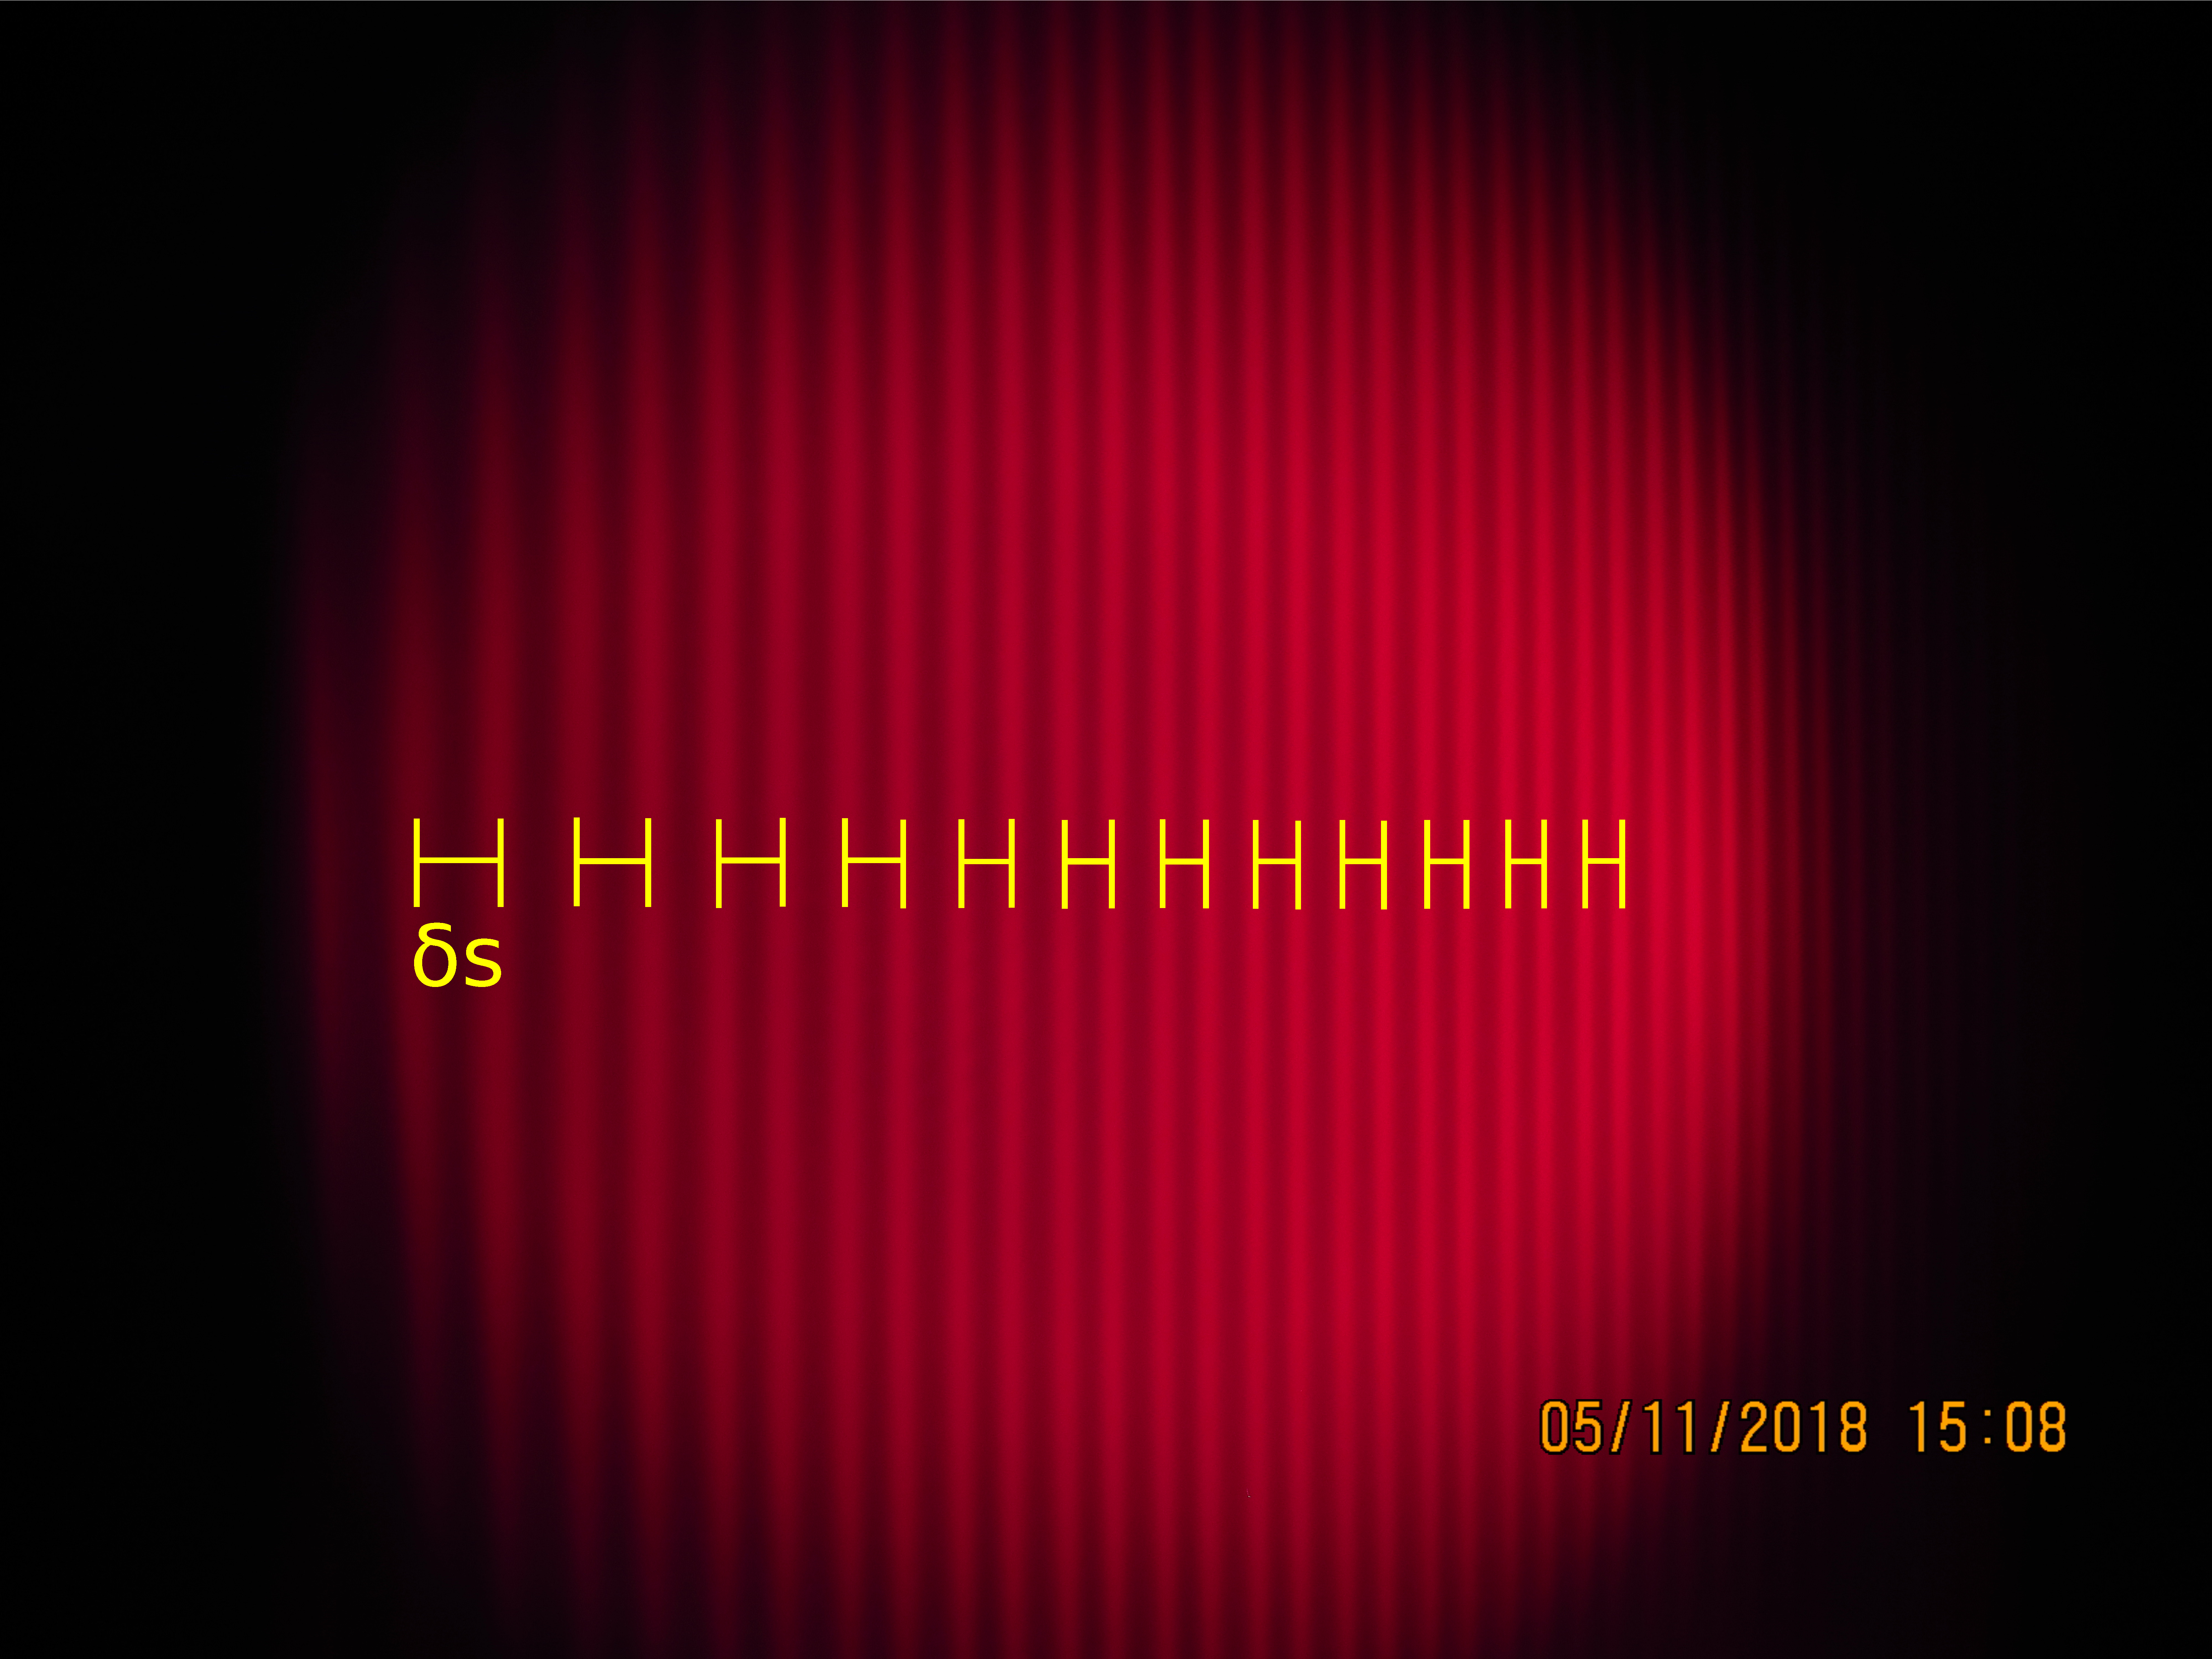
\includegraphics[height=8cm]{Experimental Pictures/red_dublett.pdf}
  \caption{Kamerabild der aufgespaltenen roten Spektrallinie bei eingeschaltetem Magnetfeld. \textit{bearbeitet}}
  \label{fig:redB}
\end{figure}

Die eingeschaltete Stromstärke für diese Aufnahme beträgt $I_\text{rot} = \SI{11.0(2)}{\ampere}$
woraus sich mittels der Parameter \eqref{eqn:kalibparams} eine Flussdichte von
\begin{align}
  B_\text{rot} = \SI{634(28)}{\milli\tesla}
\end{align}
ergibt. Analog zu oben resultieren Abstände mit einem Fehler von etwa $14 \, \text{LE}$. Diese sind
in Tabelle \ref{tab:redB} mit der jeweiligen Ordnung dargestellt. Hierbei ist darauf zu achten, dass
die Ordnung der aufgespaltenen Spektrallinie korrekt zur Ordnung der unaufgespalteten Spektrallinie
aus Abbildung \ref{tab:redB0} zugeordnet wird.

Die Messwerte $\Delta s$ und $\delta s$ inklusive berechneter Fehler sind in Abbildung \ref{fig:redds} graphisch
aufgetragen. Es fällt zum einen auf, dass die Messwerte nicht linear absinken,
und zum anderen, dass $\Delta s$ bei allen Ordnungen in etwa doppelt so groß wie $\delta s$
ist, wie es auch erwünscht ist um eine möglichst genaue Messung zu garantieren.

\begin{figure}[H]
  \centering
  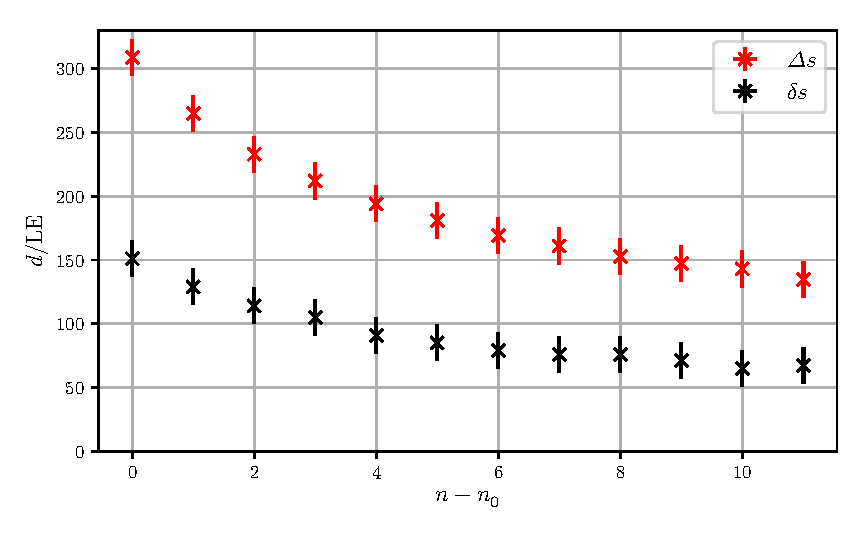
\includegraphics{build/red_ds.pdf}
  \caption{Abstandsmesswerte $\Delta s$ und $\delta s$ der roten Spektrallinie in Abhängigkeit von der Ordnung $n-n_0$.}
  \label{fig:redds}
\end{figure}

Die Quotienten $\delta s/\Delta s$ sind tabellarisch in \ref{tab:redquot} und ebenso
graphisch in Abbildung \ref{fig:redquot} eingetragen.

\begin{figure}[H]
  \centering
  \includegraphics{build/red_quot.pdf}
  \caption{Quotienten $\delta s/\Delta s$ der roten Spektrallinie in Abhängigkeit von der Ordnung $n-n_0$.}
  \label{fig:redquot}
\end{figure}

Im nächsten Schritt werden die Quotienten aller Ordnungen gemittelt, wobei sich
\begin{align}
  \left(\frac{\delta s}{\Delta s}\right)_\text{rot} = \num{0.481(26)}
\end{align}
ergibt. Die gesamte Formel für den zu berechnenden Landéschen Faktor soll hier noch
einmal angegeben werden:
\begin{align}
  g_{J,\text{rot}} = \frac{c h}{2 \mu_\text{B}} \frac{\lambda_\text{D,rot}}{B_\text{rot} \lambda_\text{rot}^2} \left(\frac{\delta s}{\Delta s}\right)_\text{rot}.
\end{align}
Die Wellenlänge $\lambda_\text{rot}$ und das Dispersionsgebiet $\lambda_\text{D,rot}$ sind in Abschnitt \ref{sec:default}
zu finden. Einsetzen aller Größen liefert den Landéschen Faktor der roten Spektrallinie
\begin{align}
  g_{J,\text{rot}} = \num{0.96(7)}.
\end{align}
Der Theoriewert lautet
\begin{align}
  g_{J,\text{rot,theorie}} = 1,
\end{align}
siehe Abschnitt \ref{sec:default} für Genaueres zur Berechnung dieses Werts.

\subsection{Ausmessung der blauen Spektrallinien}

Die Ausmessung der blauen Zeeman-Aufspaltung verläuft ähnlich zu Abschnitt \ref{sec:rotspektr}
mit dem Unterschied, dass hier zwei unterschiedliche Linien, die $\pi$- und die $\sigma$- Linie,
untersucht werden. Das bearbeitete Kamerabild der blauen Spektrallinie bei ausgeschaltetem Magnetfeld
ist in Abbildung \ref{fig:blueB0} zu sehen, während die ermittelten Abstandsmesswerte in Tabelle \ref{tab:blueB0}
aufgelistet sind. Erneut ergibt sich ein einheitlicher Fehler von etwa $14 \, \text{LE}$ bei den
Abständen.

\begin{figure}[H]
  \centering
  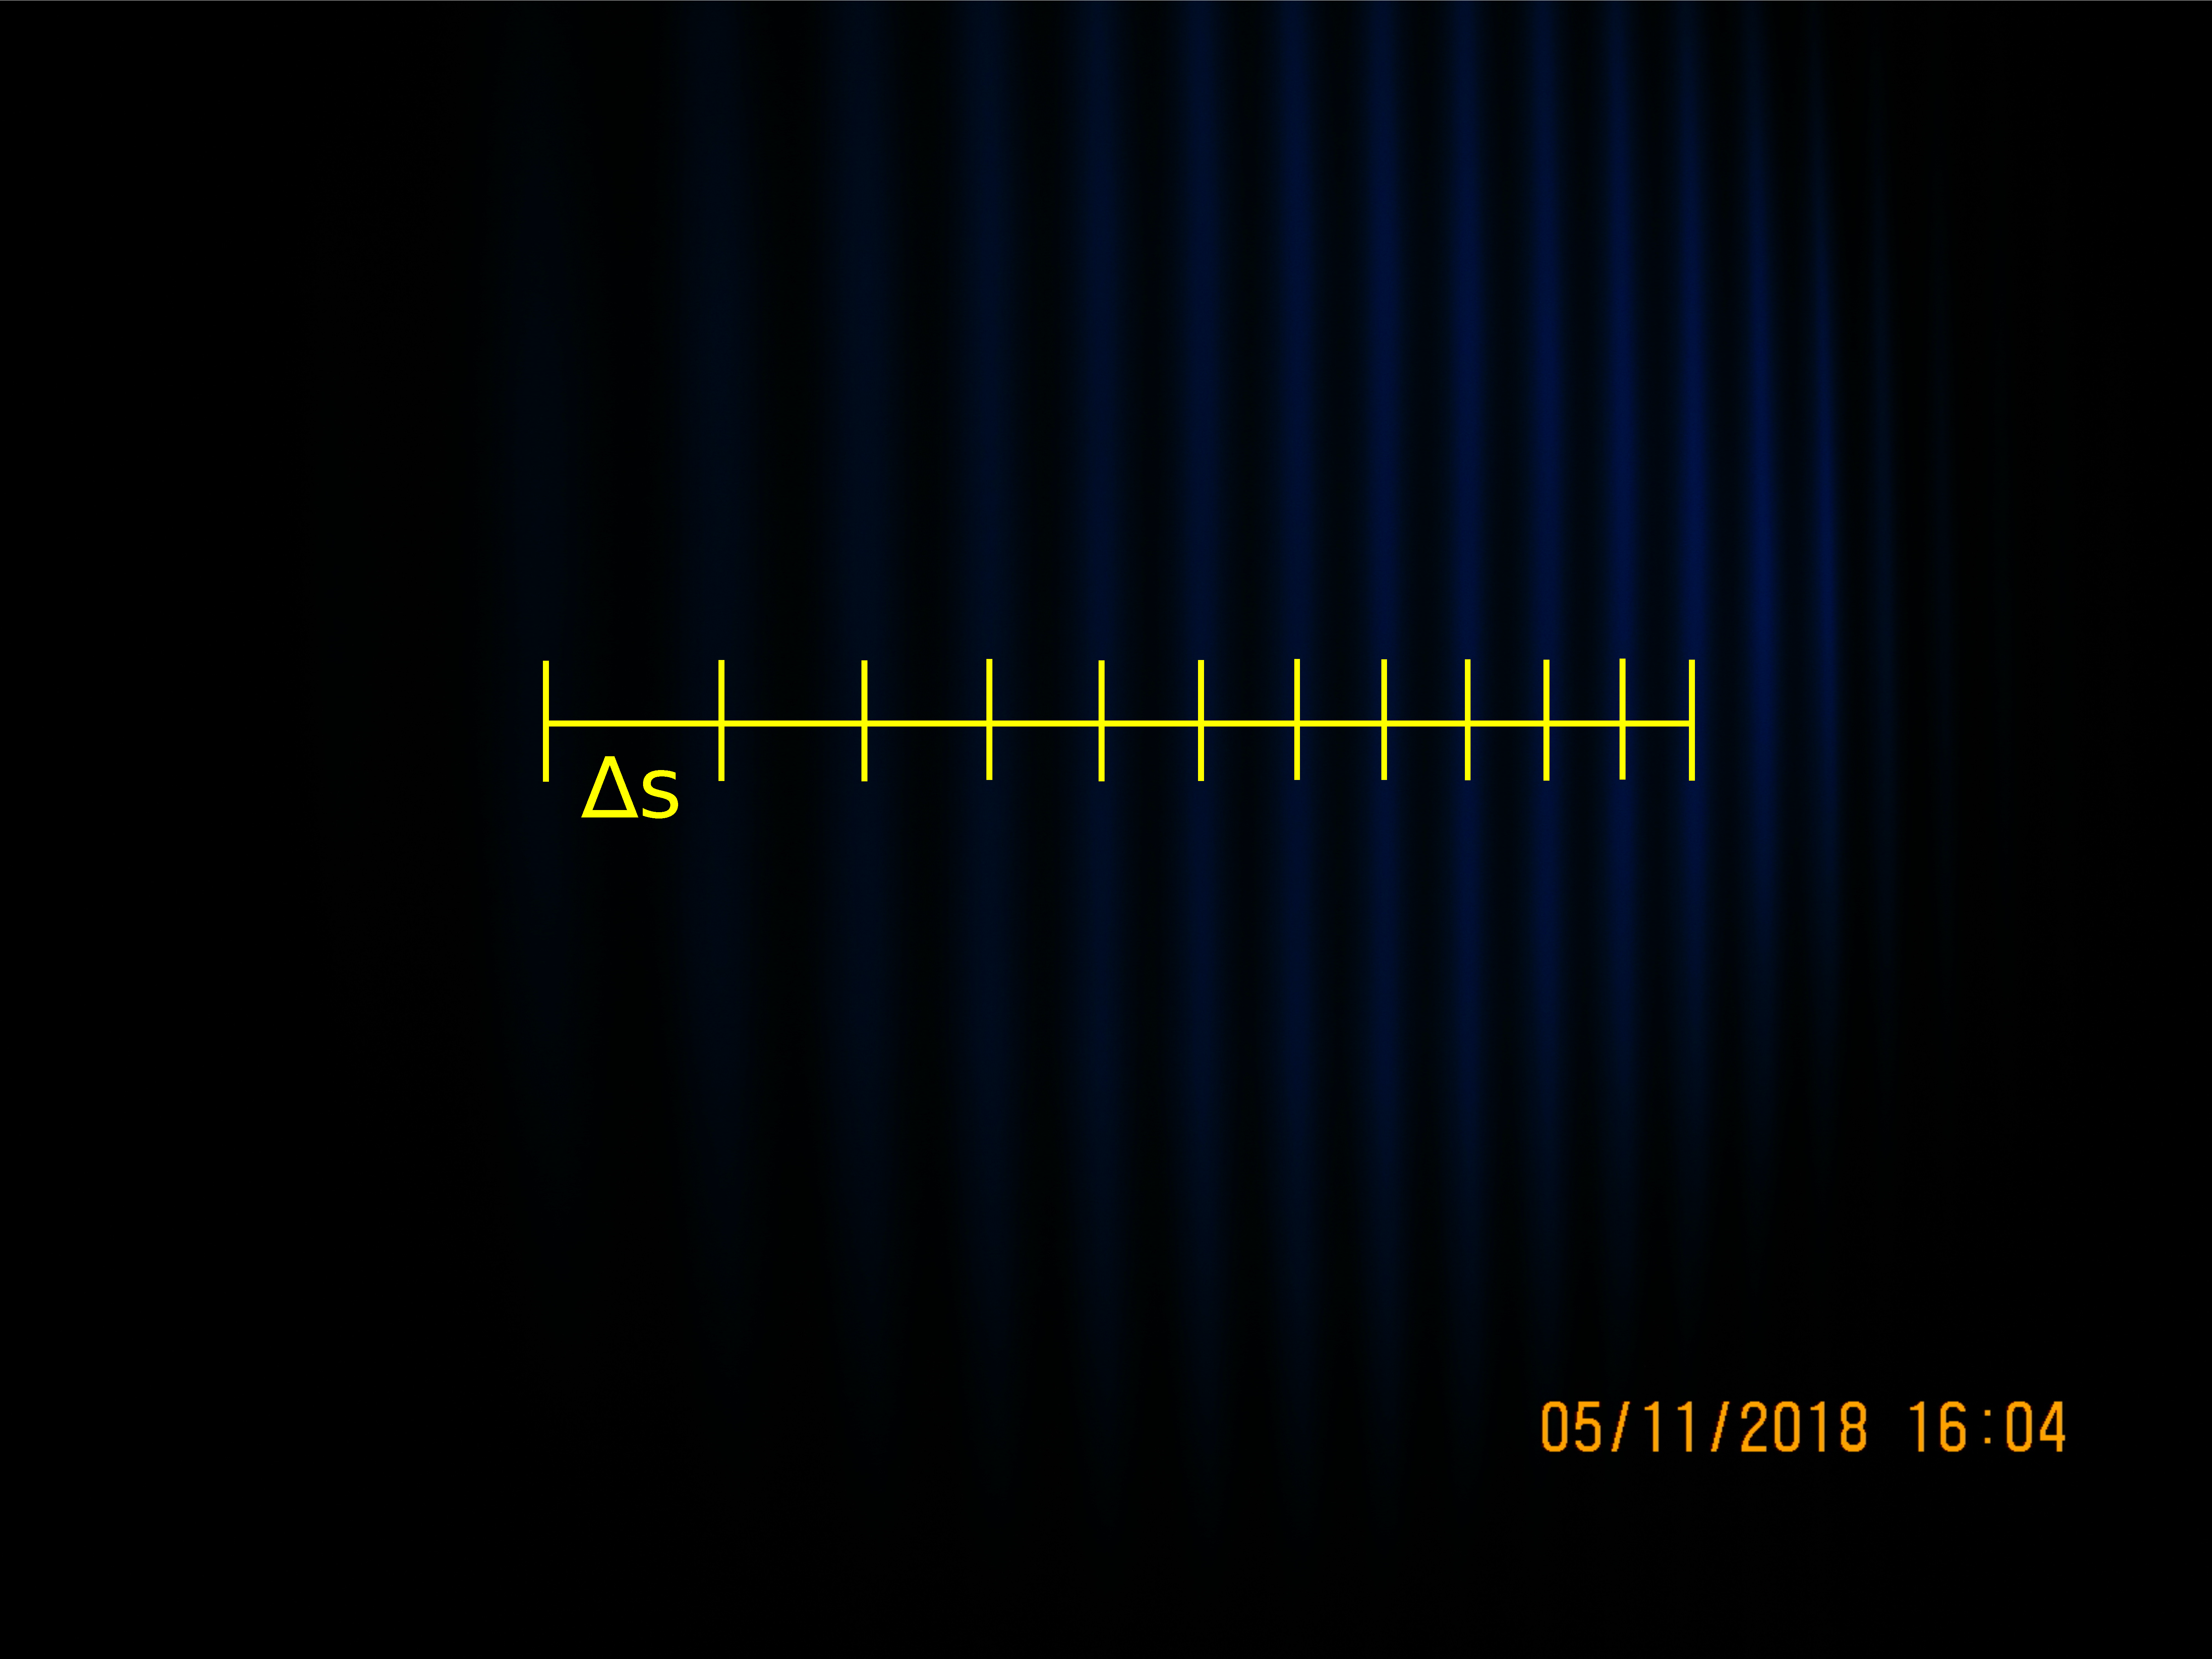
\includegraphics[height=8cm]{Experimental Pictures/blue_norm.pdf}
  \caption{Quotient $\delta s/\Delta s$ der blauen Spektrallinie in Abhängigkeit von der Ordnung $n-n_0$.}
  \label{fig:blueB0}
\end{figure}

Die bearbeiteten Kamerabilder der blauen $\pi$- und $\sigma$-Linien bei eingeschaltetem
Magnetfeld sind in den Abbildungen \ref{fig:bluepi} und \ref{fig:bluesigma} aufgezeigt.

\begin{figure}[H]
  \centering
  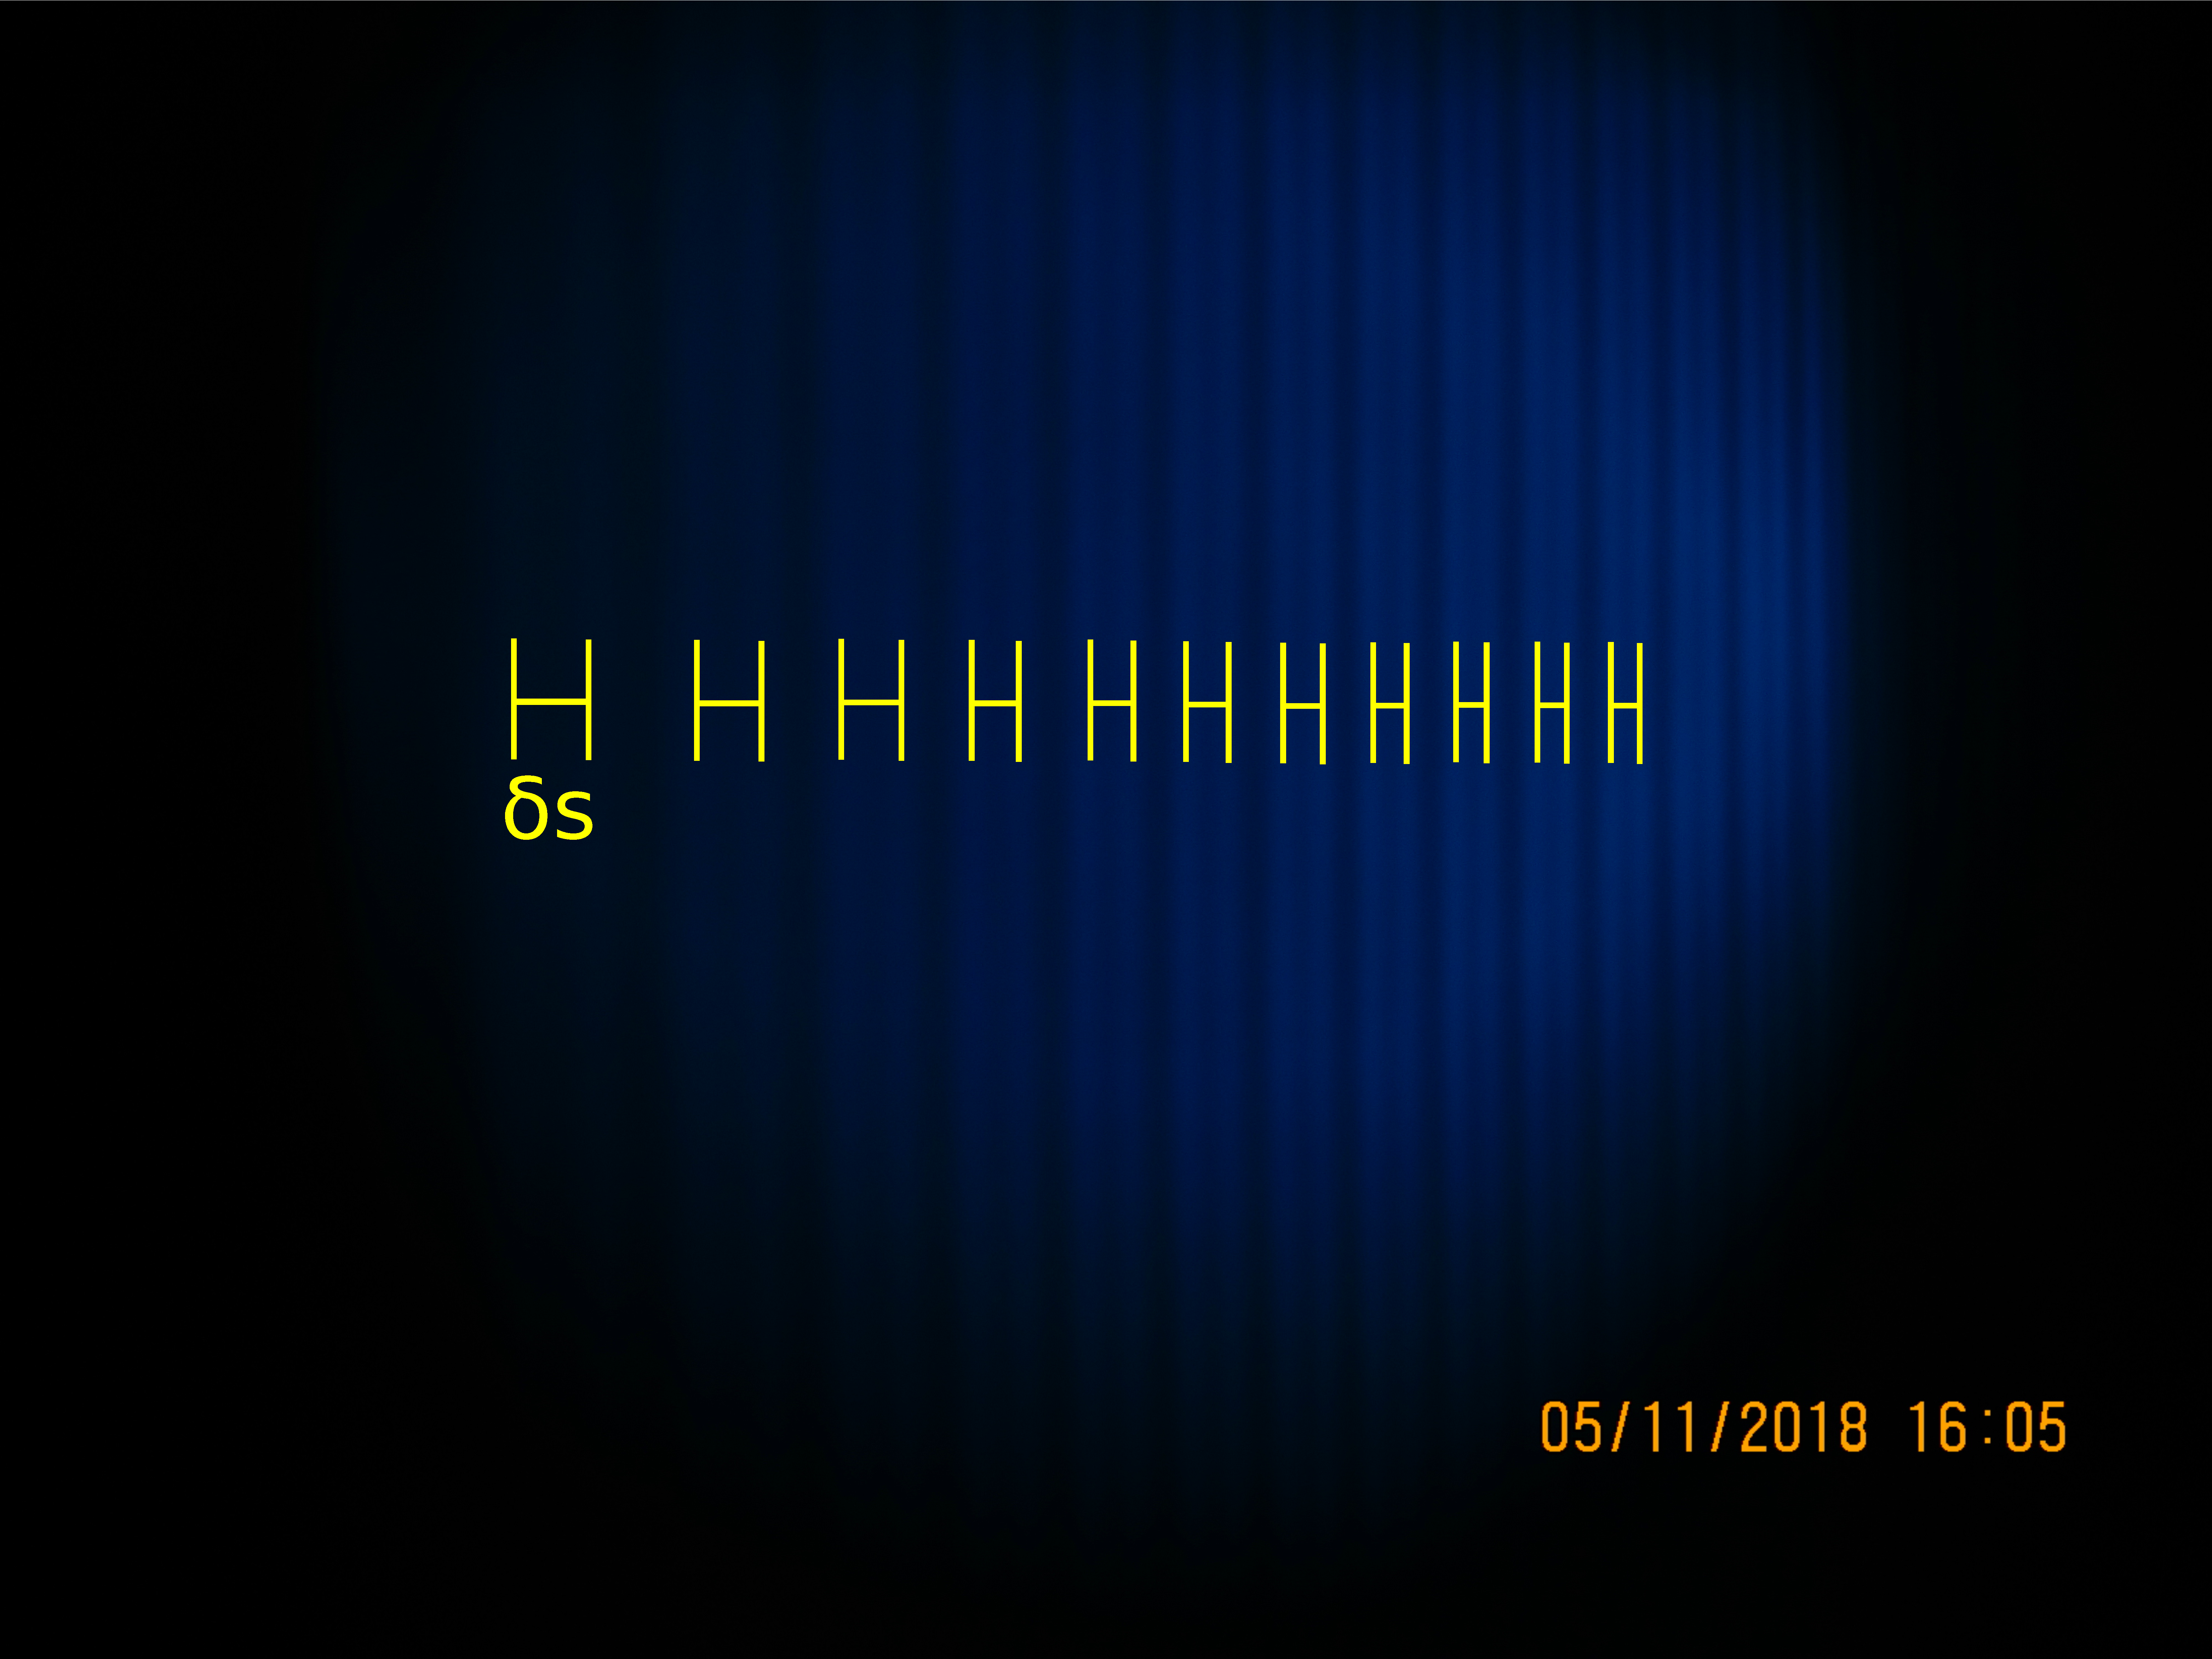
\includegraphics[height=8cm]{Experimental Pictures/blue_dublett_1.pdf}
  \caption{Kamerabild der aufgespalteten blauen $\pi$-Spektrallinie. \textit{bearbeitet}}
  \label{fig:bluepi}
\end{figure}

\begin{figure}[H]
  \centering
  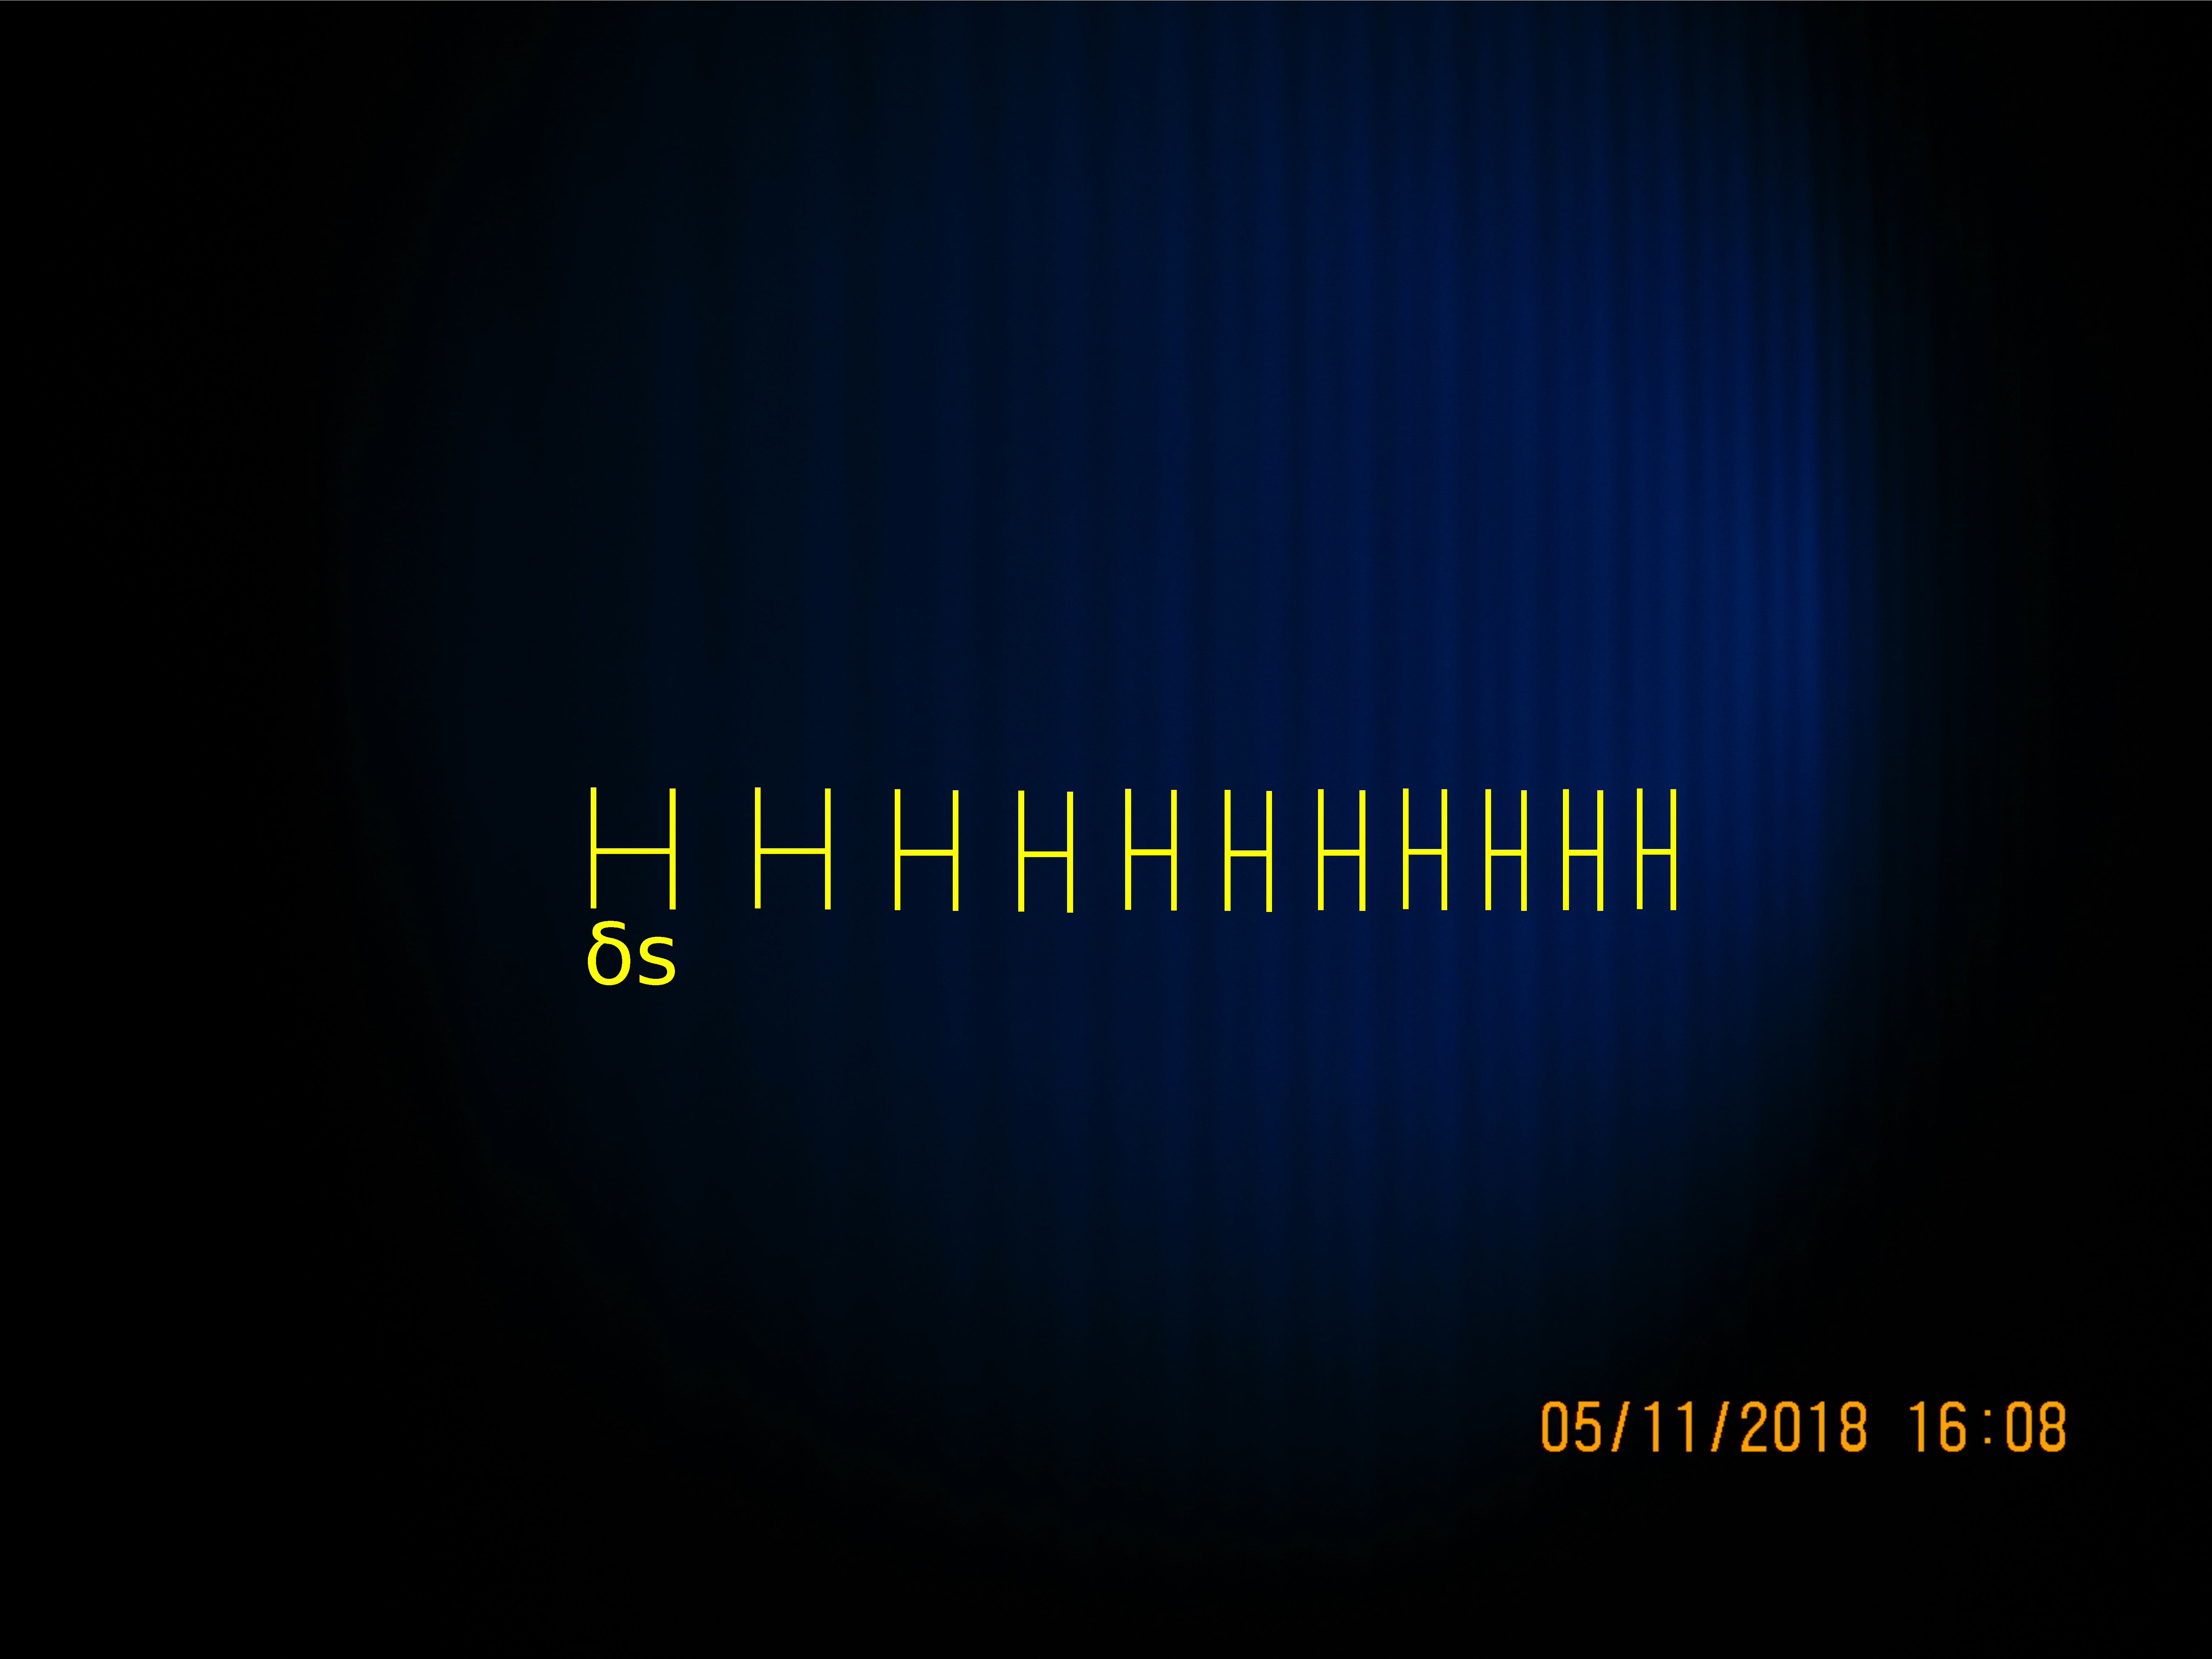
\includegraphics[height=8cm]{Experimental Pictures/blue_dublett_2.pdf}
  \caption{Kamerabild der aufgespalteten blauen $\sigma$-Spektrallinie. \textit{bearbeitet}}
  \label{fig:bluesigma}
\end{figure}

Aus den eingestellten Stromstärkewerten am Elektromagneten
\begin{align}
  I_\pi &= \SI{19.0(2)}{\ampere} & I_\sigma &= \SI{5.9(2)}{\ampere}
\end{align}
werden die Magnetfeldmesswerte analog wie in Abschnitt \ref{sec:rotspektr} mit
den Parametern aus Gleichung \ref{eqn:kalibparams} ermittelt. Es resultiert
\begin{align}
  B_\pi &= \SI{1.07(4)e3}{\milli\tesla} & B_\sigma &= \SI{360(24)}{\milli\tesla}.
  \label{eqn:Bblau}
\end{align}
Die aus den Abbildungen \ref{fig:bluepi} und \ref{fig:bluesigma} kalkulierten Abstandsmesswerte
sind ebenfalls fehlerbehaftet mit etwa $14 \, \text{LE}$ und sind in Tabelle
\ref{tab:blueBpiandsigma} und in Abbildung \ref{fig:blueds} eingetragen.

\begin{figure}[H]
  \centering
  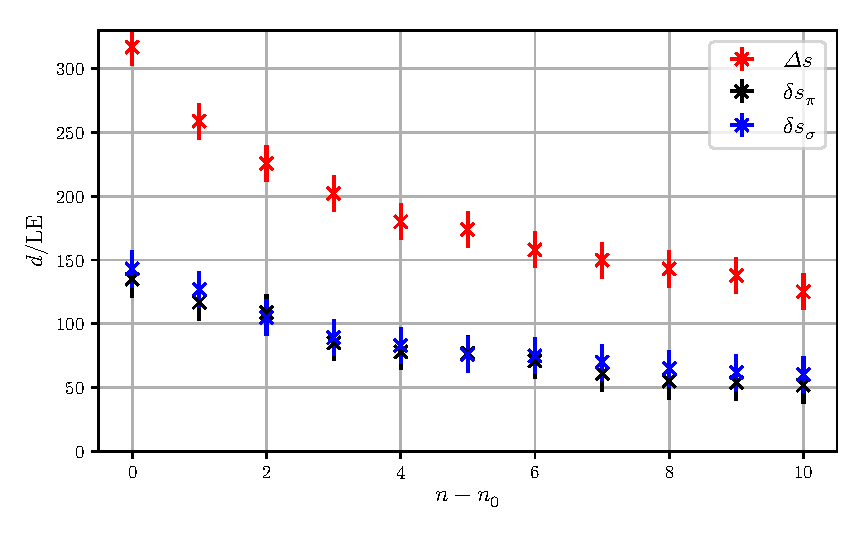
\includegraphics{build/blue_ds.pdf}
  \caption{Abstandsmesswerte $\Delta s$ und $\delta s$ der blauen $\pi$- und $\sigma$-Spektrallinie in Abhängigkeit von der Ordnung $n-n_0$.}
  \label{fig:blueds}
\end{figure}

Erneut fällt auf, dass die Abstände nicht linear mit der Ordnung absinken und die Dublettabstände $\delta s$ in etwa
halb so groß wie die Abstände $\Delta s$ sind, wie erwünscht. Weiterhin sichtbar ist, dass $\delta s_\pi$ im Durchschnitt
leicht unter $\delta s_\sigma$ liegt. Das ist dadurch begründet, dass der eingestellte $\pi$-Magnetfeldwert aus
Gleichung \eqref{eqn:Bblau} nicht der bestmögliche Wert zur Ausmessung der Spektrallinien ist, weil die Einspeisestromstärke
für den Elektromagneten nach oben begrenzt ist.

Die Quotienten $\delta s/\Delta s$ für $\pi$- und $\sigma$-Linie sind tabellarisch in \ref{tab:bluequot} und ebenso
graphisch in Abbildung \ref{fig:bluequot} eingetragen.

\begin{figure}[H]
  \centering
  \includegraphics{build/blue_quot.pdf}
  \caption{Quotienten $\delta s/\Delta s$ der blauen $\pi$- und $\sigma$-Spektrallinie in Abhängigkeit von der Ordnung $n-n_0$.}
  \label{fig:bluequot}
\end{figure}

Es errechnen sich die Mittelwerte
\begin{align}
  \left(\frac{\delta s}{\Delta s}\right)_\pi &= \num{0.428(27)} & \left(\frac{\delta s}{\Delta s}\right)_\sigma &= \num{0.461(28)}.
\end{align}
Die Formel zur Berechnung der Landéfaktoren lautet
\begin{align}
  g_{J,\pi/\sigma} = \frac{c h}{2 \mu_\text{B}} \frac{\lambda_\text{D,blau}}{B_{\pi/\sigma} \lambda_\text{blau}^2} \left(\frac{\delta s}{\Delta s}\right)_{\pi/\sigma}.
\end{align}
Damit resultiert der Landéfaktor der $\pi$-Spektrallinie
\begin{align}
  g_{J,\pi} = \num{0.50(4)}
\end{align}
und der Landéfaktor der $\sigma$-Spektrallinie
\begin{align}
  g_{J,\sigma} = \num{1.60(14)}.
\end{align}
Die Theoriewerte der Landéfaktoren lauten
\begin{align}
  g_{J,\pi,\text{theorie}} = 0.5
\end{align}
für die $\pi$-Spektrallinie und
\begin{align}
  g_{J,\sigma,\text{theorie,I}} &= 1.5 & g_{J,\sigma,\text{theorie,II}} &= 2
\end{align}
für die $\sigma$-Spektrallinie(n). Letztere können bei den Aufnahmen nicht unterschieden
werden, da sie zu nahe aneinander liegen. Daher sollte zur Bestätigung der Theorie in der
Praxis der Mittelwert
\begin{align}
  \bar{g}_{J,\sigma,\text{theorie}} = 1.75
\end{align}
gemessen werden.
